% Options for packages loaded elsewhere
\PassOptionsToPackage{unicode}{hyperref}
\PassOptionsToPackage{hyphens}{url}
%
\documentclass[
  man]{apa6}
\usepackage{amsmath,amssymb}
\usepackage{iftex}
\ifPDFTeX
  \usepackage[T1]{fontenc}
  \usepackage[utf8]{inputenc}
  \usepackage{textcomp} % provide euro and other symbols
\else % if luatex or xetex
  \usepackage{unicode-math} % this also loads fontspec
  \defaultfontfeatures{Scale=MatchLowercase}
  \defaultfontfeatures[\rmfamily]{Ligatures=TeX,Scale=1}
\fi
\usepackage{lmodern}
\ifPDFTeX\else
  % xetex/luatex font selection
\fi
% Use upquote if available, for straight quotes in verbatim environments
\IfFileExists{upquote.sty}{\usepackage{upquote}}{}
\IfFileExists{microtype.sty}{% use microtype if available
  \usepackage[]{microtype}
  \UseMicrotypeSet[protrusion]{basicmath} % disable protrusion for tt fonts
}{}
\makeatletter
\@ifundefined{KOMAClassName}{% if non-KOMA class
  \IfFileExists{parskip.sty}{%
    \usepackage{parskip}
  }{% else
    \setlength{\parindent}{0pt}
    \setlength{\parskip}{6pt plus 2pt minus 1pt}}
}{% if KOMA class
  \KOMAoptions{parskip=half}}
\makeatother
\usepackage{xcolor}
\usepackage{graphicx}
\makeatletter
\def\maxwidth{\ifdim\Gin@nat@width>\linewidth\linewidth\else\Gin@nat@width\fi}
\def\maxheight{\ifdim\Gin@nat@height>\textheight\textheight\else\Gin@nat@height\fi}
\makeatother
% Scale images if necessary, so that they will not overflow the page
% margins by default, and it is still possible to overwrite the defaults
% using explicit options in \includegraphics[width, height, ...]{}
\setkeys{Gin}{width=\maxwidth,height=\maxheight,keepaspectratio}
% Set default figure placement to htbp
\makeatletter
\def\fps@figure{htbp}
\makeatother
\setlength{\emergencystretch}{3em} % prevent overfull lines
\providecommand{\tightlist}{%
  \setlength{\itemsep}{0pt}\setlength{\parskip}{0pt}}
\setcounter{secnumdepth}{-\maxdimen} % remove section numbering
% Make \paragraph and \subparagraph free-standing
\ifx\paragraph\undefined\else
  \let\oldparagraph\paragraph
  \renewcommand{\paragraph}[1]{\oldparagraph{#1}\mbox{}}
\fi
\ifx\subparagraph\undefined\else
  \let\oldsubparagraph\subparagraph
  \renewcommand{\subparagraph}[1]{\oldsubparagraph{#1}\mbox{}}
\fi
% definitions for citeproc citations
\NewDocumentCommand\citeproctext{}{}
\NewDocumentCommand\citeproc{mm}{%
  \begingroup\def\citeproctext{#2}\cite{#1}\endgroup}
\makeatletter
 % allow citations to break across lines
 \let\@cite@ofmt\@firstofone
 % avoid brackets around text for \cite:
 \def\@biblabel#1{}
 \def\@cite#1#2{{#1\if@tempswa , #2\fi}}
\makeatother
\newlength{\cslhangindent}
\setlength{\cslhangindent}{1.5em}
\newlength{\csllabelwidth}
\setlength{\csllabelwidth}{3em}
\newenvironment{CSLReferences}[2] % #1 hanging-indent, #2 entry-spacing
 {\begin{list}{}{%
  \setlength{\itemindent}{0pt}
  \setlength{\leftmargin}{0pt}
  \setlength{\parsep}{0pt}
  % turn on hanging indent if param 1 is 1
  \ifodd #1
   \setlength{\leftmargin}{\cslhangindent}
   \setlength{\itemindent}{-1\cslhangindent}
  \fi
  % set entry spacing
  \setlength{\itemsep}{#2\baselineskip}}}
 {\end{list}}
\usepackage{calc}
\newcommand{\CSLBlock}[1]{\hfill\break\parbox[t]{\linewidth}{\strut\ignorespaces#1\strut}}
\newcommand{\CSLLeftMargin}[1]{\parbox[t]{\csllabelwidth}{\strut#1\strut}}
\newcommand{\CSLRightInline}[1]{\parbox[t]{\linewidth - \csllabelwidth}{\strut#1\strut}}
\newcommand{\CSLIndent}[1]{\hspace{\cslhangindent}#1}
\ifLuaTeX
\usepackage[bidi=basic]{babel}
\else
\usepackage[bidi=default]{babel}
\fi
\babelprovide[main,import]{english}
% get rid of language-specific shorthands (see #6817):
\let\LanguageShortHands\languageshorthands
\def\languageshorthands#1{}
% Manuscript styling
\usepackage{upgreek}
\captionsetup{font=singlespacing,justification=justified}

% Table formatting
\usepackage{longtable}
\usepackage{lscape}
% \usepackage[counterclockwise]{rotating}   % Landscape page setup for large tables
\usepackage{multirow}		% Table styling
\usepackage{tabularx}		% Control Column width
\usepackage[flushleft]{threeparttable}	% Allows for three part tables with a specified notes section
\usepackage{threeparttablex}            % Lets threeparttable work with longtable

% Create new environments so endfloat can handle them
% \newenvironment{ltable}
%   {\begin{landscape}\centering\begin{threeparttable}}
%   {\end{threeparttable}\end{landscape}}
\newenvironment{lltable}{\begin{landscape}\centering\begin{ThreePartTable}}{\end{ThreePartTable}\end{landscape}}

% Enables adjusting longtable caption width to table width
% Solution found at http://golatex.de/longtable-mit-caption-so-breit-wie-die-tabelle-t15767.html
\makeatletter
\newcommand\LastLTentrywidth{1em}
\newlength\longtablewidth
\setlength{\longtablewidth}{1in}
\newcommand{\getlongtablewidth}{\begingroup \ifcsname LT@\roman{LT@tables}\endcsname \global\longtablewidth=0pt \renewcommand{\LT@entry}[2]{\global\advance\longtablewidth by ##2\relax\gdef\LastLTentrywidth{##2}}\@nameuse{LT@\roman{LT@tables}} \fi \endgroup}

% \setlength{\parindent}{0.5in}
% \setlength{\parskip}{0pt plus 0pt minus 0pt}

% Overwrite redefinition of paragraph and subparagraph by the default LaTeX template
% See https://github.com/crsh/papaja/issues/292
\makeatletter
\renewcommand{\paragraph}{\@startsection{paragraph}{4}{\parindent}%
  {0\baselineskip \@plus 0.2ex \@minus 0.2ex}%
  {-1em}%
  {\normalfont\normalsize\bfseries\itshape\typesectitle}}

\renewcommand{\subparagraph}[1]{\@startsection{subparagraph}{5}{1em}%
  {0\baselineskip \@plus 0.2ex \@minus 0.2ex}%
  {-\z@\relax}%
  {\normalfont\normalsize\itshape\hspace{\parindent}{#1}\textit{\addperi}}{\relax}}
\makeatother

\makeatletter
\usepackage{etoolbox}
\patchcmd{\maketitle}
  {\section{\normalfont\normalsize\abstractname}}
  {\section*{\normalfont\normalsize\abstractname}}
  {}{\typeout{Failed to patch abstract.}}
\patchcmd{\maketitle}
  {\section{\protect\normalfont{\@title}}}
  {\section*{\protect\normalfont{\@title}}}
  {}{\typeout{Failed to patch title.}}
\makeatother

\usepackage{xpatch}
\makeatletter
\xapptocmd\appendix
  {\xapptocmd\section
    {\addcontentsline{toc}{section}{\appendixname\ifoneappendix\else~\theappendix\fi\\: #1}}
    {}{\InnerPatchFailed}%
  }
{}{\PatchFailed}
\keywords{meta theory, theory formation, cumulative science, formal models\newline\indent Word count: 2657}
\DeclareDelayedFloatFlavor{ThreePartTable}{table}
\DeclareDelayedFloatFlavor{lltable}{table}
\DeclareDelayedFloatFlavor*{longtable}{table}
\makeatletter
\renewcommand{\efloat@iwrite}[1]{\immediate\expandafter\protected@write\csname efloat@post#1\endcsname{}}
\makeatother
\usepackage{lineno}

\linenumbers
\usepackage{csquotes}
\ifLuaTeX
  \usepackage{selnolig}  % disable illegal ligatures
\fi
\usepackage{bookmark}
\IfFileExists{xurl.sty}{\usepackage{xurl}}{} % add URL line breaks if available
\urlstyle{same}
\hypersetup{
  pdftitle={FAIR Theory: Applying Open Science Principles to the Construction and Iterative Improvement of Scientific Theories},
  pdfauthor={Caspar J. Van Lissa1, Aaron Peikert2,3, Andreas M. Brandmaier2,3,4, \& Felix Schönbrodt5},
  pdflang={en-EN},
  pdfkeywords={meta theory, theory formation, cumulative science, formal models},
  hidelinks,
  pdfcreator={LaTeX via pandoc}}

\title{FAIR Theory: Applying Open Science Principles to the Construction and Iterative Improvement of Scientific Theories}
\author{Caspar J. Van Lissa\textsuperscript{1}, Aaron Peikert\textsuperscript{2,3}, Andreas M. Brandmaier\textsuperscript{2,3,4}, \& Felix Schönbrodt\textsuperscript{5}}
\date{}


\shorttitle{FAIR THEORY}

\authornote{

This is a preprint paper, generated from Git Commit \# d1a82fc7.

The authors made the following contributions. Caspar J. Van Lissa: Conceptualization, Formal Analysis, Funding acquisition, Methodology, Project administration, Software, Supervision, Writing -- original draft, Writing -- review \& editing; Aaron Peikert: Formal Analysis, Writing -- original draft, Writing -- review \& editing; Andreas M. Brandmaier: Formal Analysis, Writing -- original draft, Writing -- review \& editing; Felix Schönbrodt: Conceptualization, Writing -- review \& editing.

Correspondence concerning this article should be addressed to Caspar J. Van Lissa, Professor Cobbenhagenlaan 125, 5037 DB Tilburg, The Netherlands. E-mail: \href{mailto:c.j.vanlissa@tilburguniversity.edu}{\nolinkurl{c.j.vanlissa@tilburguniversity.edu}}

}

\affiliation{\vspace{0.5cm}\textsuperscript{1} Tilburg University, dept. Methodology \& Statistics\\\textsuperscript{2} Center for Lifespan Psychology, Max Planck Institute for Human Development, Berlin, Germany\\\textsuperscript{3} Max Planck UCL Centre for Computational Psychiatry and Ageing Research, Berlin, Germany\\\textsuperscript{4} Department of Psychology, MSB Medical School Berlin, Berlin, Germany\\\textsuperscript{5} Other affiliations}

\abstract{%
Test test.
}



\begin{document}
\maketitle

The FAIR Guiding Principles (hereafter: FAIR principles) were established to make research data more Findable, Accessible, Interoperable and Reusable {[}REF{]}.
Since their inception, scholars have demonstrated their relevance for making other digital research artefacts more open.
This paper argues that the FAIR principles can advance effective and transparent scholarly communication about theory as well.
To this end, we introduce ``FAIR theory'':
a digital representation of theory compliant with the FAIR principles.
FAIR Theory has the potential to substantially advance the efficiency of scholarly communication and accelerate cumulative knowledge acquisition.

The ``replication crisis'' has prompted extensive reforms in social science (Lavelle, 2021; Scheel, 2022).
Concern that undisclosed flexibility in analyses was to blame for the abundance of false-positive findings led to widespread adoption of open science practices like preregistration and replication (Nosek et al., 2015).
But have these reforms met their goal?
Recent reviews show that most preregistered hypothesis tests are not supported (Scheel, Schijen, \& Lakens, 2021).
One plausible explanation is that the replication crisis is symptomatic of an underlying,
and more fundamental, ``theory crisis''.
If psychological theories are insufficiently precise to derive testable hypotheses,
or sufficiently vague to explain contradictory findings,
then preregistration and replication will only serve to highlight those shortcomings.

Scholars have raised concerns about the state of theory in social science for nearly 50 years (Meehl, 1978; Robinaugh, Haslbeck, Ryan, Fried, \& Waldorp, 2021).
One contributing factor is a lack of theory formalization:
social scientific theories often lack the precision and clarity of theories in the physical sciences (Szollosi \& Donkin, 2021).
A second factor, which received less attention, is the a lack of transparent and democratic scholarly communication about psychological theory.
The present paper seeks to advance transparent communication about theory by applying open science principles to psychological theory for the first time,
and introducing the concept of \emph{FAIR Theory}.

FAIR Theory incorporates theory into open science workflows,
facilitates scholarly communication about theories,
making it easier to share theories with less opportunity for ambiguity and misunderstanding.
FAIR Theories are easier to find, and facilitate sharing, reusing, and updating open theories.
More efficient and transparent communication about theory democratizes and accelerates cumulative knowledge acquisition,
removes barriers for knowledge exchange with the global scholarly community,
opens theory development to diverse perspectives, and enables (distributed and adversarial) collaboration.

\subsection{Theory and Scientific Progress}\label{theory-and-scientific-progress}

According to the \emph{empirical cycle} (de Groot, 1961),
a philosophical model of cumulative knowledge acquisition,
research ideally follows a cyclical process with two phases (Figure \ref{fig:figec}).
In the deductive phase, hypotheses derived from theory are tested on data. In the inductive phase, patterns observed in data are generalized to theoretical principles.
In this model, theories are the vehicle of scientists' understanding of phenomena.
Ideally, they are iteratively updated based on deductive testing and inductive theory construction.

\begin{figure}
\centering
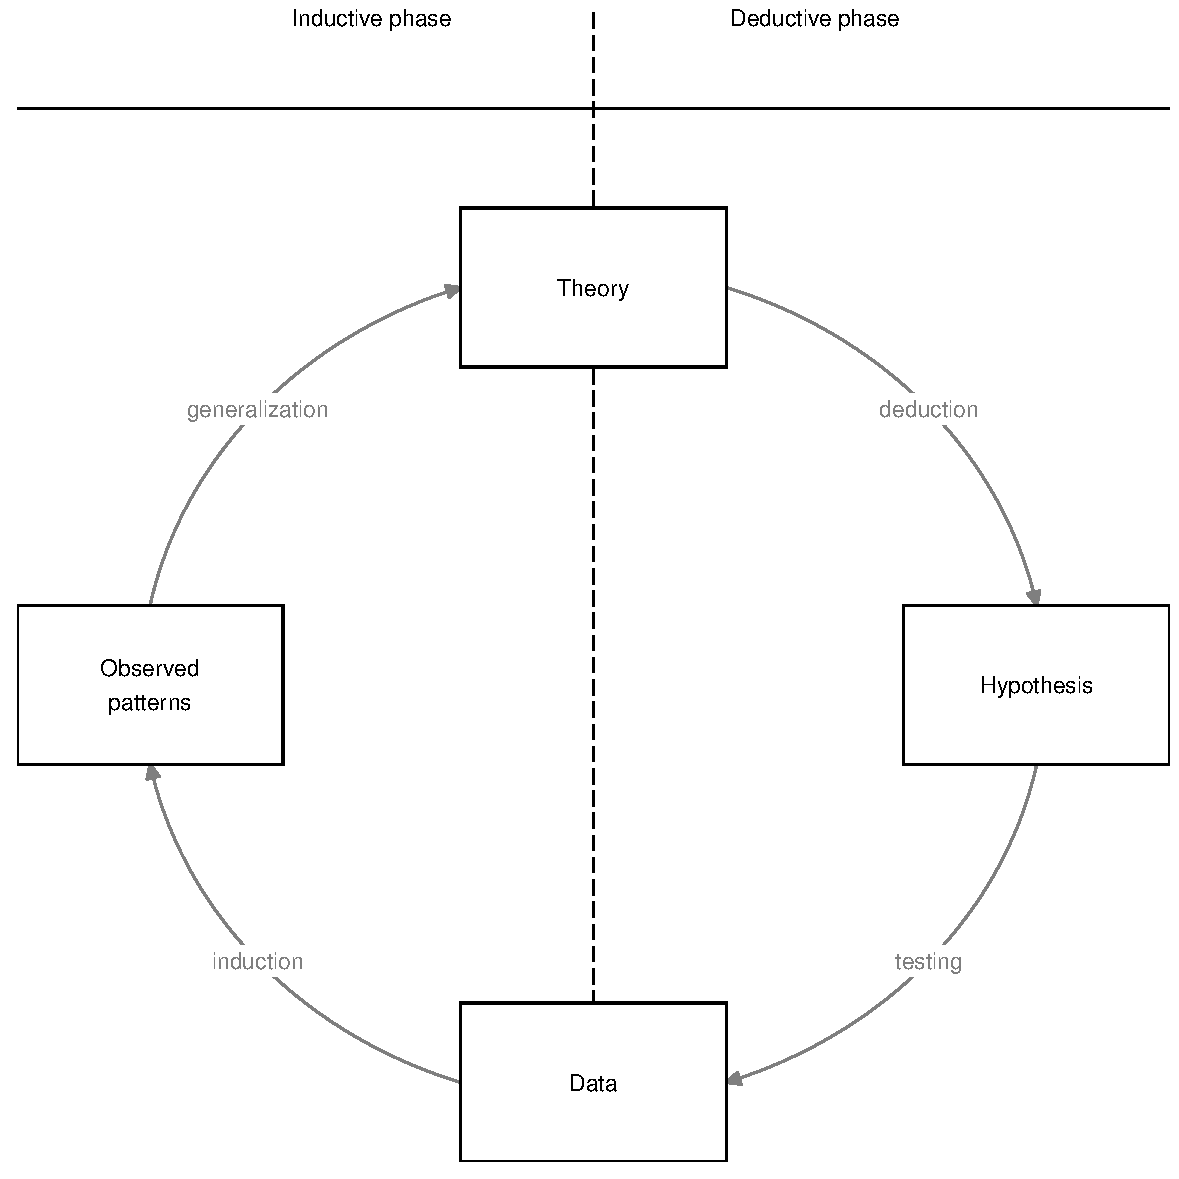
\includegraphics{empirical_cycle.pdf}
\caption{\label{fig:figec}A take on the empirical cycle by De Groot}
\end{figure}

In a progressive research program (Lakatos, 1971),
the cycle is regularly completed to iteratively advance our understanding of the studied phenomena.
There are clear indications that contemporary psychology falls short of this idealized model, however.
Firstly, because deductive research is over-represented in the literature.
According to one estimate, 89.6\% of published studies tests hypotheses,
which suggests that the literature is predominantly comprised of deductive research (Kühberger, Fritz, \& Scherndl, 2014).
Closer examination reveals, however, that the link between theory and hypothesis is often tenuous (Oberauer \& Lewandowsky, 2019; Scheel, Tiokhin, Isager, \& Lakens, 2021).
Only 15\% of deductive studies reference theory at all (McPhetres et al., 2021).
This raises the question where the other hypotheses come from,
and what consequence their refutation would have for theory.
These statistics suggest that theory has an uncomfortable and paradoxical role in contemporary psychology:
The majority of papers ostensibly test hypotheses,
but these are rarely derived from theory,
and test results rarely contribute to the improvement of existing theories.
Consequently, theories either persist unchanged for decades, or are forgotten {[}REF Meehl{]}.

Scientific reform initiated by the open science movement has predominanty focused on improving deductive methods, overlooking the shortcomings of theory.
The present paper applies, for the first time, open science principles to theory.

\subsection{Publication is not Enough}\label{publication-is-not-enough}

Merely publishing a theory does not make it open;
to be open, theory should adhere to established open science standards.
The FAIR principles, initially introduced as a standard for open research data, have since been applied to other forms of digital scholarly output (e.g., software Lamprecht et al., 2019).
We propose to apply the FAIR principles to digital representations of theory as well,
introducing a FAIR metadata format to represent (formal) theories.
The resulting theories are made \emph{Findable} via a DOI,
Accessible in a machine- and human-readable filetype,
Interoperable within the data analysis environment,
and Reusable in the practical and legal sense, so that they may be improved over time.

\subsection{Adapting the FAIR Principles}\label{adapting-the-fair-principles}

The FAIR Principles were devised to make scholarly data more findable, accessible, interoperable, and reusable.
From their inception, these principles were developed with ``other research resources'' in mind.
Scholars have translated the FAIR principles to, e.g., research software {[}REF Lamprecht{]}.
The present paper further extends the FAIR principles' definition to theory, see Table \ref{tab:tabfair}.

\begin{lltable}

\begin{longtable}{m{.1\linewidth}m{.35\linewidth}m{.35\linewidth}m{.15\linewidth}m{.1\linewidth}m{.35\linewidth}m{.35\linewidth}m{.15\linewidth}m{.1\linewidth}m{.35\linewidth}m{.35\linewidth}m{.15\linewidth}m{.1\linewidth}m{.35\linewidth}m{.35\linewidth}m{.15\linewidth}}\noalign{\getlongtablewidth\global\LTcapwidth=\longtablewidth}
\caption{\label{tab:tabfair}}\\
\toprule
Criterion & \multicolumn{1}{c}{Original} & \multicolumn{1}{c}{Theory} & \multicolumn{1}{c}{Action}\\
\midrule
\endfirsthead
\caption*{\normalfont{Table \ref{tab:tabfair} continued}}\\
\toprule
Criterion & \multicolumn{1}{c}{Original} & \multicolumn{1}{c}{Theory} & \multicolumn{1}{c}{Action}\\
\midrule
\endhead
F1 & (Meta)data are assigned a globally unique and persistent identifier & Theory and its associated metadata has a global, unique and persistent identifier for each version (using semantic versioning) & Rephrased\\
F2 & Data are described with rich metadata & Theory is described with rich metadata & \textasciitilde{}same\\
F3 & Metadata clearly and explicitly include the identifier of the data it describes & Metadata clearly and explicitly include identifiers for all the versions of the theory it describes & \textasciitilde{}same\\
F4 & (Meta)data are registered or indexed in a searchable resource & Theory and its associated metadata are included in a searchable repository & NEEDS WORK! GitHub is indexed by Google I believe, but ideally, we'd like our theories to show up in Google Scholar, or even dedicated academic search enginges. Where could we put them to realize this?\\
A1 & (Meta)data are retrievable by their identifier using a standardized communications protocol & Theory and its associated metadata are accessible by their identifier using a standardized communications protocol & \textasciitilde{}same\\
A1.1 & The protocol is open, free, and universally implementable & The protocol is open, free, and universally implementable & Same\\
A1.2 & The protocol allows for an authentication and authorization procedure, where necessary & The protocol allows for an authentication and authorization procedure, where necessary & Do\ \ we need this?\\
A2 & Metadata are accessible, even when the data are no longer available & Theory metadata are accessible, even when the theory is no longer available & Do\ \ we need this?\\
I1 & (Meta)data use a formal, accessible, shared, and broadly applicable language for knowledge representation & Theory and its associated metadata use a formal, accessible, shared and broadly applicable language to facilitate machine readability and reuse & Rephrased\\
I2 & (Meta)data use vocabularies that follow FAIR principles & (Meta)data use vocabularies that follow FAIR principles & NEEDS WORK! I think this is where we explain the value of e.g. universal graph languages like Aaron and Max'\\
I2S.1 & - &  & \\
I2S.2 & - &  & \\
I3 & (Meta)data include qualified references to other (meta)data & (Meta)data includes qualified references to other (meta)data, including previous versions of the theory & Rephrased. I envision a LinkList-like structure where each theory version references its ancestor\\
I4S & - &  & Discard\\
R1 & (Meta)data are richly described with a plurality of accurate and relevant attributes & Theory and its associated metadata are richly described with a plurality of accurate and relevant attributes & Needs work. How do we envision this? Keywords? ISBN-like codes for variable type?\\
R1.1 & (Meta)data are released with a clear and accessible data usage license & (Meta)data are released with a clear and accessible license & Needs work: which license is good for theory?\\
R1.2 & (Meta)data are associated with detailed provenance & (Meta)data are associated with detailed provenance & Relates to I3; I think this point relates more to the theory's ancestry, and I3 relates to e.g. incorporating other theories within a theory (e.g., theory of measurement inside of structural theory)\\
R1.3 & (Meta)data meet domain-relevant community standards & Theory metadata and documentation meet domain-relevant community standards & These standards do not yet exist; we can take a first step towards developing them and recommend that this be an active area of development\\
\bottomrule
\end{longtable}

\end{lltable}

\subsection{Is Current Psychological Theory FAIR?}\label{is-current-psychological-theory-fair}

While a comprehensive analysis of the present state of FAIR Theory in psychology is beyond the scope of the present paper,
we provide a narrative review of examples and counterexamples for each criterion.

One factor that contributes to poor findability of psychological theory is that the primary unit of dissemination and search in psychology is the academic paper.
A paper may contain multiple resources - including materials, data, code, and theory - but there is no unified search engine for theory,
or even an agreed-upon keyword (model, framework, etc are often used interchangeably with theory).
Modular publishing could ameliorate the Findability of psychological theory.
In this approach, distinct resources are individually published as citable academic output.
Such output can still be linked; for example, a FAIR theory could have an accompanying paper.
Another effort to improve theories' findability is post-hoc curation.
For example, Gray and colleagues introduced a format for representing theories,
and post many examples on their website.
Similarly, Borsboom and colleagues seek to establish a dictionary of psychological ``phenomena'' (which are not strictly theories, but are patterns reliably evidenced by data that theory should seek to explain).

With regard to Accessibility, publishing behind paywalls certainly has a negative impact.
Open Access publishing increases the accessibility of all academic output, including theory.
Another factor curtailing the accessibility of theory is ambiguity;
a lack of theory formalization introduces a dependency on the original author for clarification.
The discourse on ``Great Man Theorizing'' touches upon the problems this introduces {[}REF Guest et al moral theory{]}.
For example, dependency on interpretation by the author creates a potential for gatekeeping - the author could insist that work requires their involvement, which violates checks and balances of scientific research.
Moreover, if a theory is refuted, its author could claim that the author of the refuting paper did not interpret the theory correctly.
To some extent, this relates to the problem of translation {[}REF Duhem{]}:
it is not possible to entirely formalize an idea to enable unambiguous interpretation.
Nonetheless, taking care to formalize a theory to the maximum extent possible advances Accessibility.

There are clear indications that psychological theory has limited interoperability.
For one, theories are rarely \emph{``refuted nor corroborated, but instead merely fade away as people lose interest''} (Meehl, 1978).
To be interoperable, psychological theory would need to play a concrete part in scientists' day-to-day work.
For example, it should be possible to integrate theory directly into analysis workflows:
to derive hypotheses, select control variables, and guide model specification.
The aforementioned lack of formalization {[}REF Robinaugh{]} and ambiguity {[}REF Frankenhuis{]} prevent interoperability in such a practical sense.
Additionally, theories should be interoperable with each other:
for instance, it should be possible to embed a specific theory about the process of emotion regulation {[}REF Gross{]} within a theory of emotion regulation development {[}REF Morris{]}.

There appears to be a norm \emph{against} the reuse of theory,
as evident from the quip that
\emph{``{[}Theories are{]} like toothbrushes --- no self-respecting person wants to use anyone else's''} (Mischel, 2008).
Moreover, a legal basis for theory reuse is often absent.
Questions that often come up in our workshops on FAIR Theory are ``who owns theory'',
and ``who determines how a theory may be changed''?
Such questions require a clear answer, even if that answer may vary across theories.
Licensing theories for reuse provides clarity about how a theory can be reused.
A crucial legal consideration is that,
while specific (FAIR) representations of theory might be protected by copyright,
the underlying ideas are not.
This is another argument in favor of publishing specific instantiations of theory along with licenses detailing how they may be reused.

\subsection{FAIR Theory and Recognition \& Rewards}\label{fair-theory-and-recognition-rewards}

In the spirit of DORA, extending the FAIR principles to theory helps researchers obtain credit for their theoretical contributions - obviating the necessity of publishing a theoretical paper, which can be challenging.
From a meta-science perspective, FAIR theory facilitates studying the state of theory in a particular subfield, and comparing theories' substantive and structural properties. Version control and cross-referencing additionally enable tracing and studying the ancestry and development of theories.

FAIR theory provides a clear deliverable, and a clear goal, for scholars and institutions seeking to promote contributions to theory.

There are key distinctions between theory and other FAIR digital research artefacts. With this in mind, following the example of Lamprecht and colleagues, we reflect on how the criteria underlying the FAIR Principles apply to theory.

\subsection{The Role of Theory Formalization}\label{the-role-of-theory-formalization}

Concerns about the state of theory are a recurring theme in the psychological literature,
but previous writing has focused on theory formalization as a solution for ambiguity in psychological theory.
Greater formality increases theories' \emph{empirical content},
making them easier to falsify,
which necessitates revising them,
thus advancing our principled understanding of the phenomena they describe.
Conceptually, theory formalization is orthogonal to FAIR theory.
FAIR Theory does not require theories to be formal, and formal theory can be represented in a way that is not FAIR.
It is - in principle - possible to represent a collection of verbal statements as a FAIR Theory.
While FAIR Theory is fully consistent with formal theory, it does not require theories to be formal.

\subsection{Version Control}\label{version-control}

\begin{itemize}
\tightlist
\item
  One source of potential improvements of theory methodology that has not been previously considered is computer science.
\item
  The process of ``iteratively improving'' digital objects - in this case, computer code - is well understood.
\item
  Recent work like the FAIR software principles has demonstrated that ideals of open science apply to computer science as well.
\item
  This paper argues that, conversely, principles of computer science - particularly version control, algorithmic hypothesis generation (find better word; this is about using the digital theory object to derive implied hypotheses), and integrated testing, can also be used to improve theory methods in the social science.
\item
  We introduce ``FAIR theory'', a digital research artifact to represent formal social scientific theories
\item
  FAIR theory can be version controlled; any time new insights require modifications of the theory, these modifications can be documented in a traceable and reversable manner. Version control also enables diffuse collaboration in theory development, as other researchers can submit ``pull requests'' to suggest modifications of a theory, or can ``fork'' existing theories to create a spin-off from an existing theory.
\end{itemize}

\section{Examples}\label{examples}

\subsection{Formalizing the Empirical Cycle}\label{formalizing-the-empirical-cycle}

In this example, we represent the empirical cycle - a theory of cumulative knowledge production through scientific research - as FAIR theory.
As several authors have taken inspiration from the work by De Groot,
we compare our interpretation of the original theory to the interpretation of others.
Originally, the theory has the following structure:

\begin{verbatim}

digraph {

  observation;
  induction;
  deduction;
  test;
  evaluation;
  
  observation -> induction;
  induction -> deduction;
  deduction -> test;
  test -> evaluation;
  evaluation -> observation;
  
}
\end{verbatim}

Subsequently, Wagenmakers and colleagues modified the theory by \emph{``{[}adding the{]} Whewell-Peirce-Reichenbach distinction between the context of discovery and the context of justification''}:

\begin{verbatim}
digraph {

  subgraph cluster_discovery {
    label="Discovery";
    hypothesis [label="New hypothesis"];
    prediction [label="New prediction"];
  }
  data  [label="Old knowledge and old data"];      
  subgraph cluster_justification {
    label="Justification";
    test [label="Test on new data"];
    evaluation;
  }

  data -> hypothesis [label="Speculate & explore"];
  hypothesis -> prediction  [label="Deduce"];
  prediction -> test  [label="Design new experiment"];
  test -> evaluation  [label="Statistical analysis"];
  evaluation -> data  [label="Knowledge accumulation"];

}
\end{verbatim}

Note, however, that there appear to be further changes:
the phases of the cycle have been renamed,
and the annotations suggest a move towards experimental empirical psychology that was absent in the original formulation.
Moreover, the label ``knowledge accumulation'' invites the question of exactly \emph{how} knowledge accumulates upon evaluation of a prior experiment.
As this lack of cumulative knowledge acquisition appears to be precisely where contemporary research practice falls short, this ambiguity invites further improvement of the theory.

Our work, too is inspired by De Groot, but our take on the empirical cycle is different again:

\begin{verbatim}
digraph {

  theory;
  prediction;
  test [label="inferential procedure"];
  observation;
  
  theory -> prediction [label="deduction"];
  prediction -> test;
  test -> observation;
  observation -> theory [label="generalization"];

}
\end{verbatim}

In our representation,
induction is not a separate phase but a mode of reasoning by which specific observations are generalized into theory.
For example, the refutation of a hypothesized effect,
or the serendipitous observation of some pattern in data,
might be a reason to revise or construct theory.
Induction, incidentally, also occurs within the link from prediction to testing:
in the form of the inductive bias of methods used to perform the test,
and auxiliary assumptions that must be made to address remaining theoretical ambiguities.

\subsection{Using FAIR Theory to Perform Causal Inference}\label{using-fair-theory-to-perform-causal-inference}

Some have argued that \emph{causal explanations} are a property of good theory {[}REF Meehl, etc?{]}.
According to Pearl and colleagues,
explicit assumptions about the direction of causality allow one to perform causal inference even on cross-sectional data.
Any formal theory that is explicit about direction of causality could thus be used to guide causal inference,
and could even be integrated into the analysis environment.

In this example, we illustrate how to use DAGs for causal inference, including the detection of a violation of the initial model and subsequent adaptation of the DAG. We could use that to illustrate updating FAIR theory:

\url{https://currentprotocols.onlinelibrary.wiley.com/doi/full/10.1002/cpz1.45}

We can find more examples of causal inference with DAGs in these tutorials:

\url{https://www.r-bloggers.com/2019/08/causal-inference-with-dags-in-r/}

\url{https://www.r-bloggers.com/2018/08/applications-of-dags-in-causal-inference/}

\begin{itemize}
\tightlist
\item
  Theory is the vehicle of cumulative knowledge acquisition
\item
  According to the empirical cycle, ideally, hypotheses are derived from theory, then tested in data, and theory is amended based on the resulting insights. When this cycle is regularly completed, theories become ever more veracious representations of social scientific phenomena.
\item
  At present, there is concern over a theory crisis in the social sciences, which highlights that this system is not functioning as intended, and highlights the need for better theory.
\item
  One source of potential improvements of theory methodology that has not been previously considered is computer science.
\item
  The process of ``iteratively improving'' digital objects - in this case, computer code - is well understood.
\item
  Recent work like the FAIR software principles has demonstrated that ideals of open science apply to computer science as well.
\item
  This paper argues that, conversely, principles of computer science - particularly version control, algorithmic hypothesis generation (find better word; this is about using the digital theory object to derive implied hypotheses), and integrated testing, can also be used to improve theory methods in the social science.
\item
  We introduce ``FAIR theory'', a digital research artifact to represent formal social scientific theories
\item
  FAIR theory can be version controlled; any time new insights require modifications of the theory, these modifications can be documented in a traceable and reversable manner. Version control also enables diffuse collaboration in theory development, as other researchers can submit ``pull requests'' to suggest modifications of a theory, or can ``fork'' existing theories to create a spin-off from an existing theory.
\item
  FAIR theory allows for algorithmic derivation of hypotheses implied by the theory.
\item
  FAIR theory enables integration testing: researchers can build a ``test suite'' of evidence that must be explainable by the theory, and any modifications of the theory must also pass the test suite.
\item
  To illustrate FAIR theory's potential to accelerate cumulative knowledge acquisition, we present several tutorial examples, developed in collaboration with applied researchers across fields of social science.
\end{itemize}

\newpage

\section{References}\label{references}

\phantomsection\label{refs}
\begin{CSLReferences}{1}{0}
\bibitem[\citeproctext]{ref-degrootMethodologieGrondslagenVan1961}
de Groot, A. D. (1961). \emph{Methodologie: Grondslagen van onderzoek en denken in de gedragswetenschappen}. 's Gravenhage: Uitgeverij Mouton. Retrieved from \url{https://books.google.com?id=6hiBDwAAQBAJ}

\bibitem[\citeproctext]{ref-kuhbergerPublicationBiasPsychology2014}
Kühberger, A., Fritz, A., \& Scherndl, T. (2014). Publication {Bias} in {Psychology}: {A Diagnosis Based} on the {Correlation} between {Effect Size} and {Sample Size}. \emph{PLoS ONE}, \emph{9}(9), e105825. \url{https://doi.org/10.1371/journal.pone.0105825}

\bibitem[\citeproctext]{ref-lakatosHistoryScienceIts1971}
Lakatos, I. (1971). History of {Science} and its {Rational Reconstructions}. In R. C. Buck \& R. S. Cohen (Eds.), \emph{{PSA} 1970: {In Memory} of {Rudolf Carnap Proceedings} of the 1970 {Biennial Meeting Philosophy} of {Science Association}} (pp. 91--136). Dordrecht: Springer Netherlands. \url{https://doi.org/10.1007/978-94-010-3142-4_7}

\bibitem[\citeproctext]{ref-lamprechtFAIRPrinciplesResearch2019}
Lamprecht, A.-L., Garcia, L., Kuzak, M., Martinez, C., Arcila, R., Martin Del Pico, E., \ldots{} Capella-Gutierrez, S. (2019). Towards {FAIR} principles for research software. \emph{Data Science}, 1--23. \url{https://doi.org/10.3233/DS-190026}

\bibitem[\citeproctext]{ref-lavelleWhenCrisisBecomes2021}
Lavelle, J. S. (2021). When a {Crisis Becomes} an {Opportunity}: {The Role} of {Replications} in {Making Better Theories}. \emph{The British Journal for the Philosophy of Science}, 714812. \url{https://doi.org/10.1086/714812}

\bibitem[\citeproctext]{ref-mcphetresDecadeTheoryReflected2021}
McPhetres, J., Albayrak-Aydemir, N., Mendes, A. B., Chow, E. C., Gonzalez-Marquez, P., Loukras, E., \ldots{} Volodko, K. (2021). A decade of theory as reflected in {Psychological Science} (2009--2019). \emph{PLOS ONE}, \emph{16}(3), e0247986. \url{https://doi.org/10.1371/journal.pone.0247986}

\bibitem[\citeproctext]{ref-meehlTheoreticalRisksTabular1978}
Meehl, P. E. (1978). Theoretical {Risks} and {Tabular Asterisks}: {Sir Karl}, {Sir Ronald}, and the {Slow Progress} of {Soft Psychology}. \emph{Journal of Consulting \& Clinical Psychology}, \emph{46}(4), 806--834.

\bibitem[\citeproctext]{ref-mischelToothbrushProblem2008}
Mischel, W. (2008). The {Toothbrush Problem}. \emph{APS Observer}, \emph{21}. Retrieved from \url{https://www.psychologicalscience.org/observer/the-toothbrush-problem}

\bibitem[\citeproctext]{ref-nosekPromotingOpenResearch2015a}
Nosek, B. A., Alter, G., Banks, G. C., Borsboom, D., Bowman, S. D., Breckler, S. J., \ldots{} Yarkoni, T. (2015). Promoting an open research culture. \emph{Science}, \emph{348}(6242), 1422--1425. \url{https://doi.org/10.1126/science.aab2374}

\bibitem[\citeproctext]{ref-oberauerAddressingTheoryCrisis2019}
Oberauer, K., \& Lewandowsky, S. (2019). Addressing the theory crisis in psychology. \emph{Psychonomic Bulletin \& Review}, \emph{26}(5), 1596--1618. \url{https://doi.org/10.3758/s13423-019-01645-2}

\bibitem[\citeproctext]{ref-robinaughInvisibleHandsFine2021}
Robinaugh, D. J., Haslbeck, J. M. B., Ryan, O., Fried, E. I., \& Waldorp, L. J. (2021). Invisible {Hands} and {Fine Calipers}: {A Call} to {Use Formal Theory} as a {Toolkit} for {Theory Construction}. \emph{Perspectives on Psychological Science}, \emph{16}(4), 725--743. \url{https://doi.org/10.1177/1745691620974697}

\bibitem[\citeproctext]{ref-scheelWhyMostPsychological2022}
Scheel, A. M. (2022). Why most psychological research findings are not even wrong. \emph{Infant and Child Development}, \emph{31}(1), e2295. \url{https://doi.org/10.1002/icd.2295}

\bibitem[\citeproctext]{ref-scheelExcessPositiveResults2021}
Scheel, A. M., Schijen, M. R. M. J., \& Lakens, D. (2021). An {Excess} of {Positive Results}: {Comparing} the {Standard Psychology Literature With Registered Reports}. \emph{Advances in Methods and Practices in Psychological Science}, \emph{4}(2), 25152459211007467. \url{https://doi.org/10.1177/25152459211007467}

\bibitem[\citeproctext]{ref-scheelWhyHypothesisTesters2021}
Scheel, A. M., Tiokhin, L., Isager, P. M., \& Lakens, D. (2021). Why {Hypothesis Testers Should Spend Less Time Testing Hypotheses}. \emph{Perspectives on Psychological Science}, \emph{16}(4), 744--755. \url{https://doi.org/10.1177/1745691620966795}

\bibitem[\citeproctext]{ref-szollosiArrestedTheoryDevelopment2021}
Szollosi, A., \& Donkin, C. (2021). Arrested theory development: {The} misguided distinction between exploratory and confirmatory research. \emph{Perspectives on Psychological Science}, \emph{16}(4), 717--724. \url{https://doi.org/10.1177/1745691620966796}

\end{CSLReferences}


\end{document}
